\documentclass[a4paper, fontsize = 14pt]{article}
\usepackage{hyperref}
\usepackage[warn]{mathtext}
\usepackage[english,russian]{babel}
\usepackage[utf8x]{inputenc} 
 
%математика
\usepackage[mathscr]{eucal}
\usepackage{amsmath,amsfonts,amssymb,amsthm,mathtools}
\usepackage{icomma}
\usepackage{wasysym}
\usepackage{mathrsfs}
 
%оформление текста
\usepackage{setspace}
\onehalfspacing
\usepackage{indentfirst}
\usepackage{scrextend}
 
%геометрия
\usepackage{geometry}
\geometry{left=25mm,right=25mm,
 top=25mm,bottom=30mm}
 
%графика
\usepackage{wrapfig}
\usepackage{graphicx}
\usepackage{pgfplots}
\usepackage{tikz}
\RequirePackage{caption}
\DeclareCaptionLabelSeparator{defffis}{ --- }
\captionsetup{justification=centering,labelsep=defffis}
 
%таблицы
\usepackage{array,tabularx,tabulary,booktabs} 
\usepackage{longtable}  
\usepackage{multirow} 
 
%ссылки
\usepackage{hyperref}
\usepackage{xcolor}
\definecolor{grn}{HTML}{57A14F} %зеленый
\definecolor{rd}{HTML}{E53C44} %красный 
\definecolor{bl}{HTML}{282691} %синий 
\definecolor{bbl}{HTML}{001B6C} %темно-синий
\hypersetup{		
    colorlinks=true,       	
    linkcolor=bbl,          % внутренние ссылки
    citecolor=rd,          % на библиографию
    filecolor=magenta,      % на файлы
    urlcolor=bl           %внешние источники
}
 
% Колонтитулы
\usepackage{fancyhdr} 
 	\pagestyle{fancy}
 	\renewcommand{\headrulewidth}{0.15mm}  
 	\renewcommand{\footrulewidth}{0.15mm}
 	\lfoot{МФТИ, 2021}
 	\rfoot{\thepage}
 	\cfoot{}
 	\rhead{}
 	\chead{}
 	\lhead{}
 
 
\begin{document}

\begin{center} \textbf{
Лабораторная работа №2.5.1 \\ Измерение коэффициента \\ поверхностного натяжения жидкости\\
Мещеряков Всеволод, Б02-001, 26.03.2021}
\end{center} 

\subsection*{Введение}

Цель этой работы состоит в измерении температурной зависимости коэффициента поверхностного натяжения дистиллированной воды с использованием известного коэффициента поверхностного натяжения спирта. Для этого используются прибор Ребиндера с термостатом и микроманометром и рабочие сосуды.

Согласно формуле Лапласа, избыточное давление внутри жидкости, создаваемое пузырьком воздуха в ней, определяется так:

\begin{equation}
	\Delta P = \frac{2\sigma}{r}.
\end{equation}

В формуле (1) $\sigma$ - коэффициент поверхностного натяжения жидкости, $\Delta P$ - избыточное давление, $r$ - радиус кривизны поверхности раздела (в нашем случае это радиус пузырька). В работе измеряется разность давлений при разных температурах, что позволяет изучить зависимость коэффициента от нее.

\subsection*{Экспериментальная установка}

\begin{figure}[hbt]\label{risI}
\center{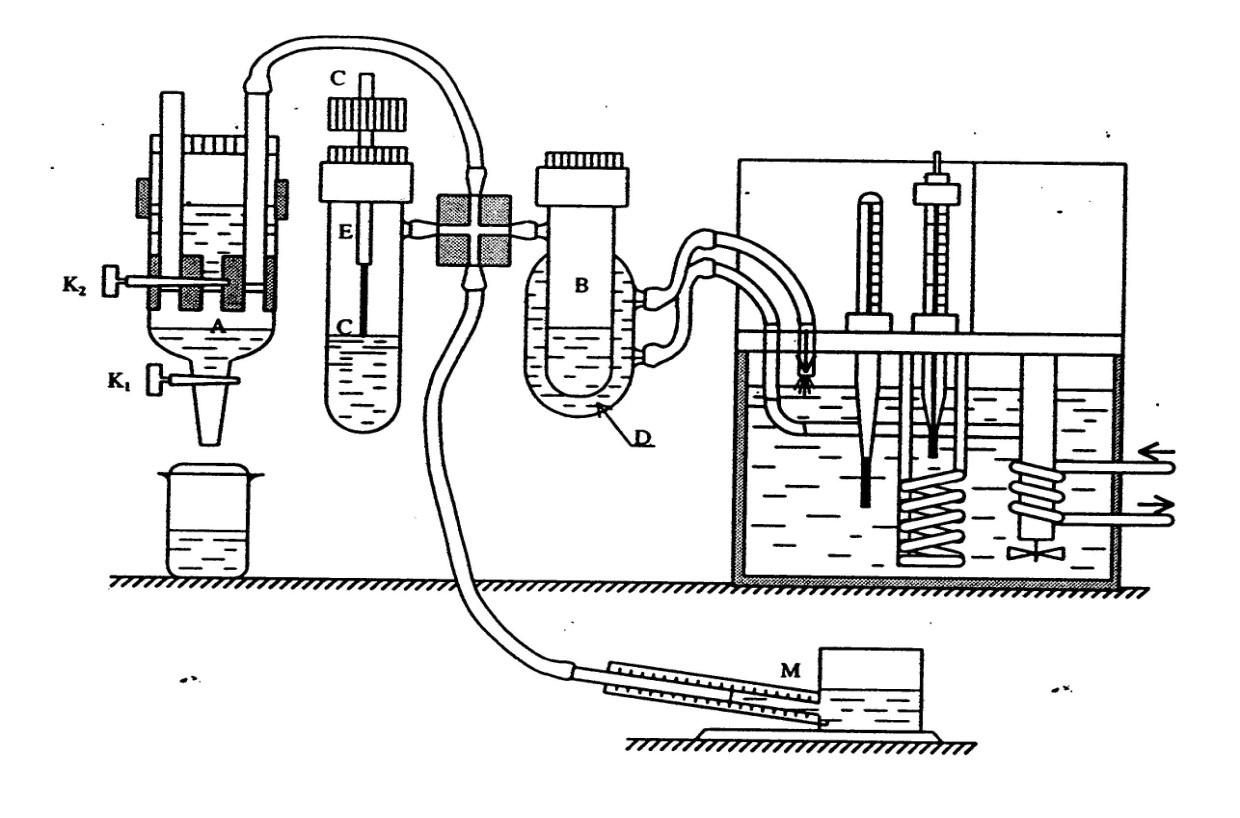
\includegraphics[scale=1.1]{lab251ris1.jpg}}
\caption{\textit{Схема установки}}
\end{figure}

Исследуемая жидкость находится в колбе В. Тестовая жидкость (в нашем случае 96$\%$ спирт) в колбе Е. В ходе работы обе они плотно закрыты, чем изолированы от внешней среды. В одну из них (в зависимости от предмета изучения) вставлена игла С, один конец которой открыт в атмосферу, а другой погружен в жидкость. При достаточном разряжении воздух из иглы пробулькивается через жидкость, что позволяет фиксировать разность давлений.

Разряжение же достигается с помощью аспиратора А. Кран К2 разделяет его на две части. Им можно контролировать количество воды (при необходимости доливать её). Открытие же крана К1 выпускает воду из полости А, что при закрытом К2 начинает разряжать всю установку. В работе исплоьзуются квазистатические приближения, поэтому, чтобы оставить их верными, вода выпускается малыми каплями не чаще, чем раз в 5 секунд. 

Давление в системе измеряется микроманометром М. Его показания переводятся в Паскали так:

\begin{equation}
	P = C \cdot h \frac{\gamma_{сп.залит}}{\gamma_{сп.пр}} \cdot K \cdot 9,81.
\end{equation}

В формуле (2) P - давление в системе, Паскали; C - поправочный множитель, определяемый наклоном манометра; $\gamma_{сп.залит}$ - плотность 96 $\%$ спирта, залитого в манометр; $\gamma_{сп.пр}$ - плотность спирта, указанная на приборе. Для используемого в работе эти конснанты равны:

$ K = 0,2 , \,\, C = 1,00, \,\, \gamma_{сп.залит} = 0,8075 \, (г/см^3) , \, \, \gamma_{сп.пр} = 0,8095 \, (г/см^3). $

При снятии температурной зависимости игла будет погружена на некоторую глубину, поэтому манометр будет показывать давление с учетом гидростатического давления столба жидкости. 

\subsection*{Ход работы}

Опустим иглу так, чтобы она только касалась поверхности тестовой жидкости (96$\%$ спирт). Откроем кран К1 так, чтобы капли падали с описанной ранее частотой. Замерим максимальное давление по формуле(2) при пробулькивании пузырьков воздуха. Из табличных значений возьмем коэффициент поверхностного натяжения для тестовой жидкости, откуда по формуле (1) определим диаметр иглы, считая, что пузырьки выходят такого же размера:

$ \Delta P_{max} = (470 \pm 5)\cdot10^{-1} (дел) \overset{(2)}{\Longrightarrow }\Delta P_{max} = (919\pm9)\cdot10^{-1}(Па)$

\[ \overset{(1)}{\Longrightarrow} r_{Л} = \frac{2 \sigma }{\Delta P_{max}} = (479\pm5)\cdot10^{-6}(м). \]

Прямые измерения микроскопом же дают $r_{М} = (475\pm3)\cdot10^{-6}(м)$, что и берется за истиное. Различие с Лапласовской формулой объясняется тем, что пузыри выходят размером не строго равным размеру иглы. 

Перенесем иглу в сосуд с дистиллированной водой. Измерим максимальное давление $P_1$ пробулькивания, когда игла лишь касается поверхности воды. $P_1 = (1400\pm5)\cdot10^{-1}(дел)\overset{(2)}{\Longrightarrow}P_1 = (2740\pm9)\cdot10^{-1}(Па)$. Также измерим высоту, на которую опустился верхний конец иглы $h_0 = (235\pm5)\cdot10^{-2}(см)$.

Погрузим иглу максимально глубоко и измерим глубину погружения. Её верхний конец оказывается на высоте $h_1 = (100\pm5)\cdot10^{-2}(см)$, из чего делаем вывод, что игла находится на глубине $h = h_0 - h_1 = (135\pm10)\cdot10^{-2}(см)$. 

Начнем снимать температурную зависимость $\sigma(T)$. Результаты измерений приведены в таблице 1 приложения. Для каждого максимального давления вычислим соответствующий $\sigma$ и по этим данным построим график $\sigma(T)$ - рисунок 3 приложения. Из него определим угол наклона полученной прямой:

\[ \frac{d\sigma(T)}{dT} = -(173\pm11)\cdot10^{-6} (\frac{Н}{м\cdot К}). \]

Построим графики $q(T)=-T\cdot\frac{d\sigma}{dT}$ - зависимость теплоты образования единицы поверхности от температуры (рис.4 приложения) и $\frac{U}{F}(T) = \sigma(T) - T\cdot\frac{d\sigma}{dT}$ - зависимость поверхностной энергии U единицы площади F от температуры (рис.5 приложения).

\subsection*{Вывод}

В этой работе была получена температурная зависимость коэффициента поверхностного натяжения $96\%$ спирта (см. стр. 4). На опыте было показано, что теоретическое приближение этой зависимости к линейной выполняется. Также график на рисунке 5 приложения показывает, что внутренняя энергия поверхности не зависит от температуры. Отклонения от табличных значений вызваны многими факторами: нечистотой изучаемого раствора спирта, различием в размерах пузырьков и иглы, неидеальностью работы манометра.

\subsection*{Приложение}

\begin{figure}[hbt]\label{risI}
\center{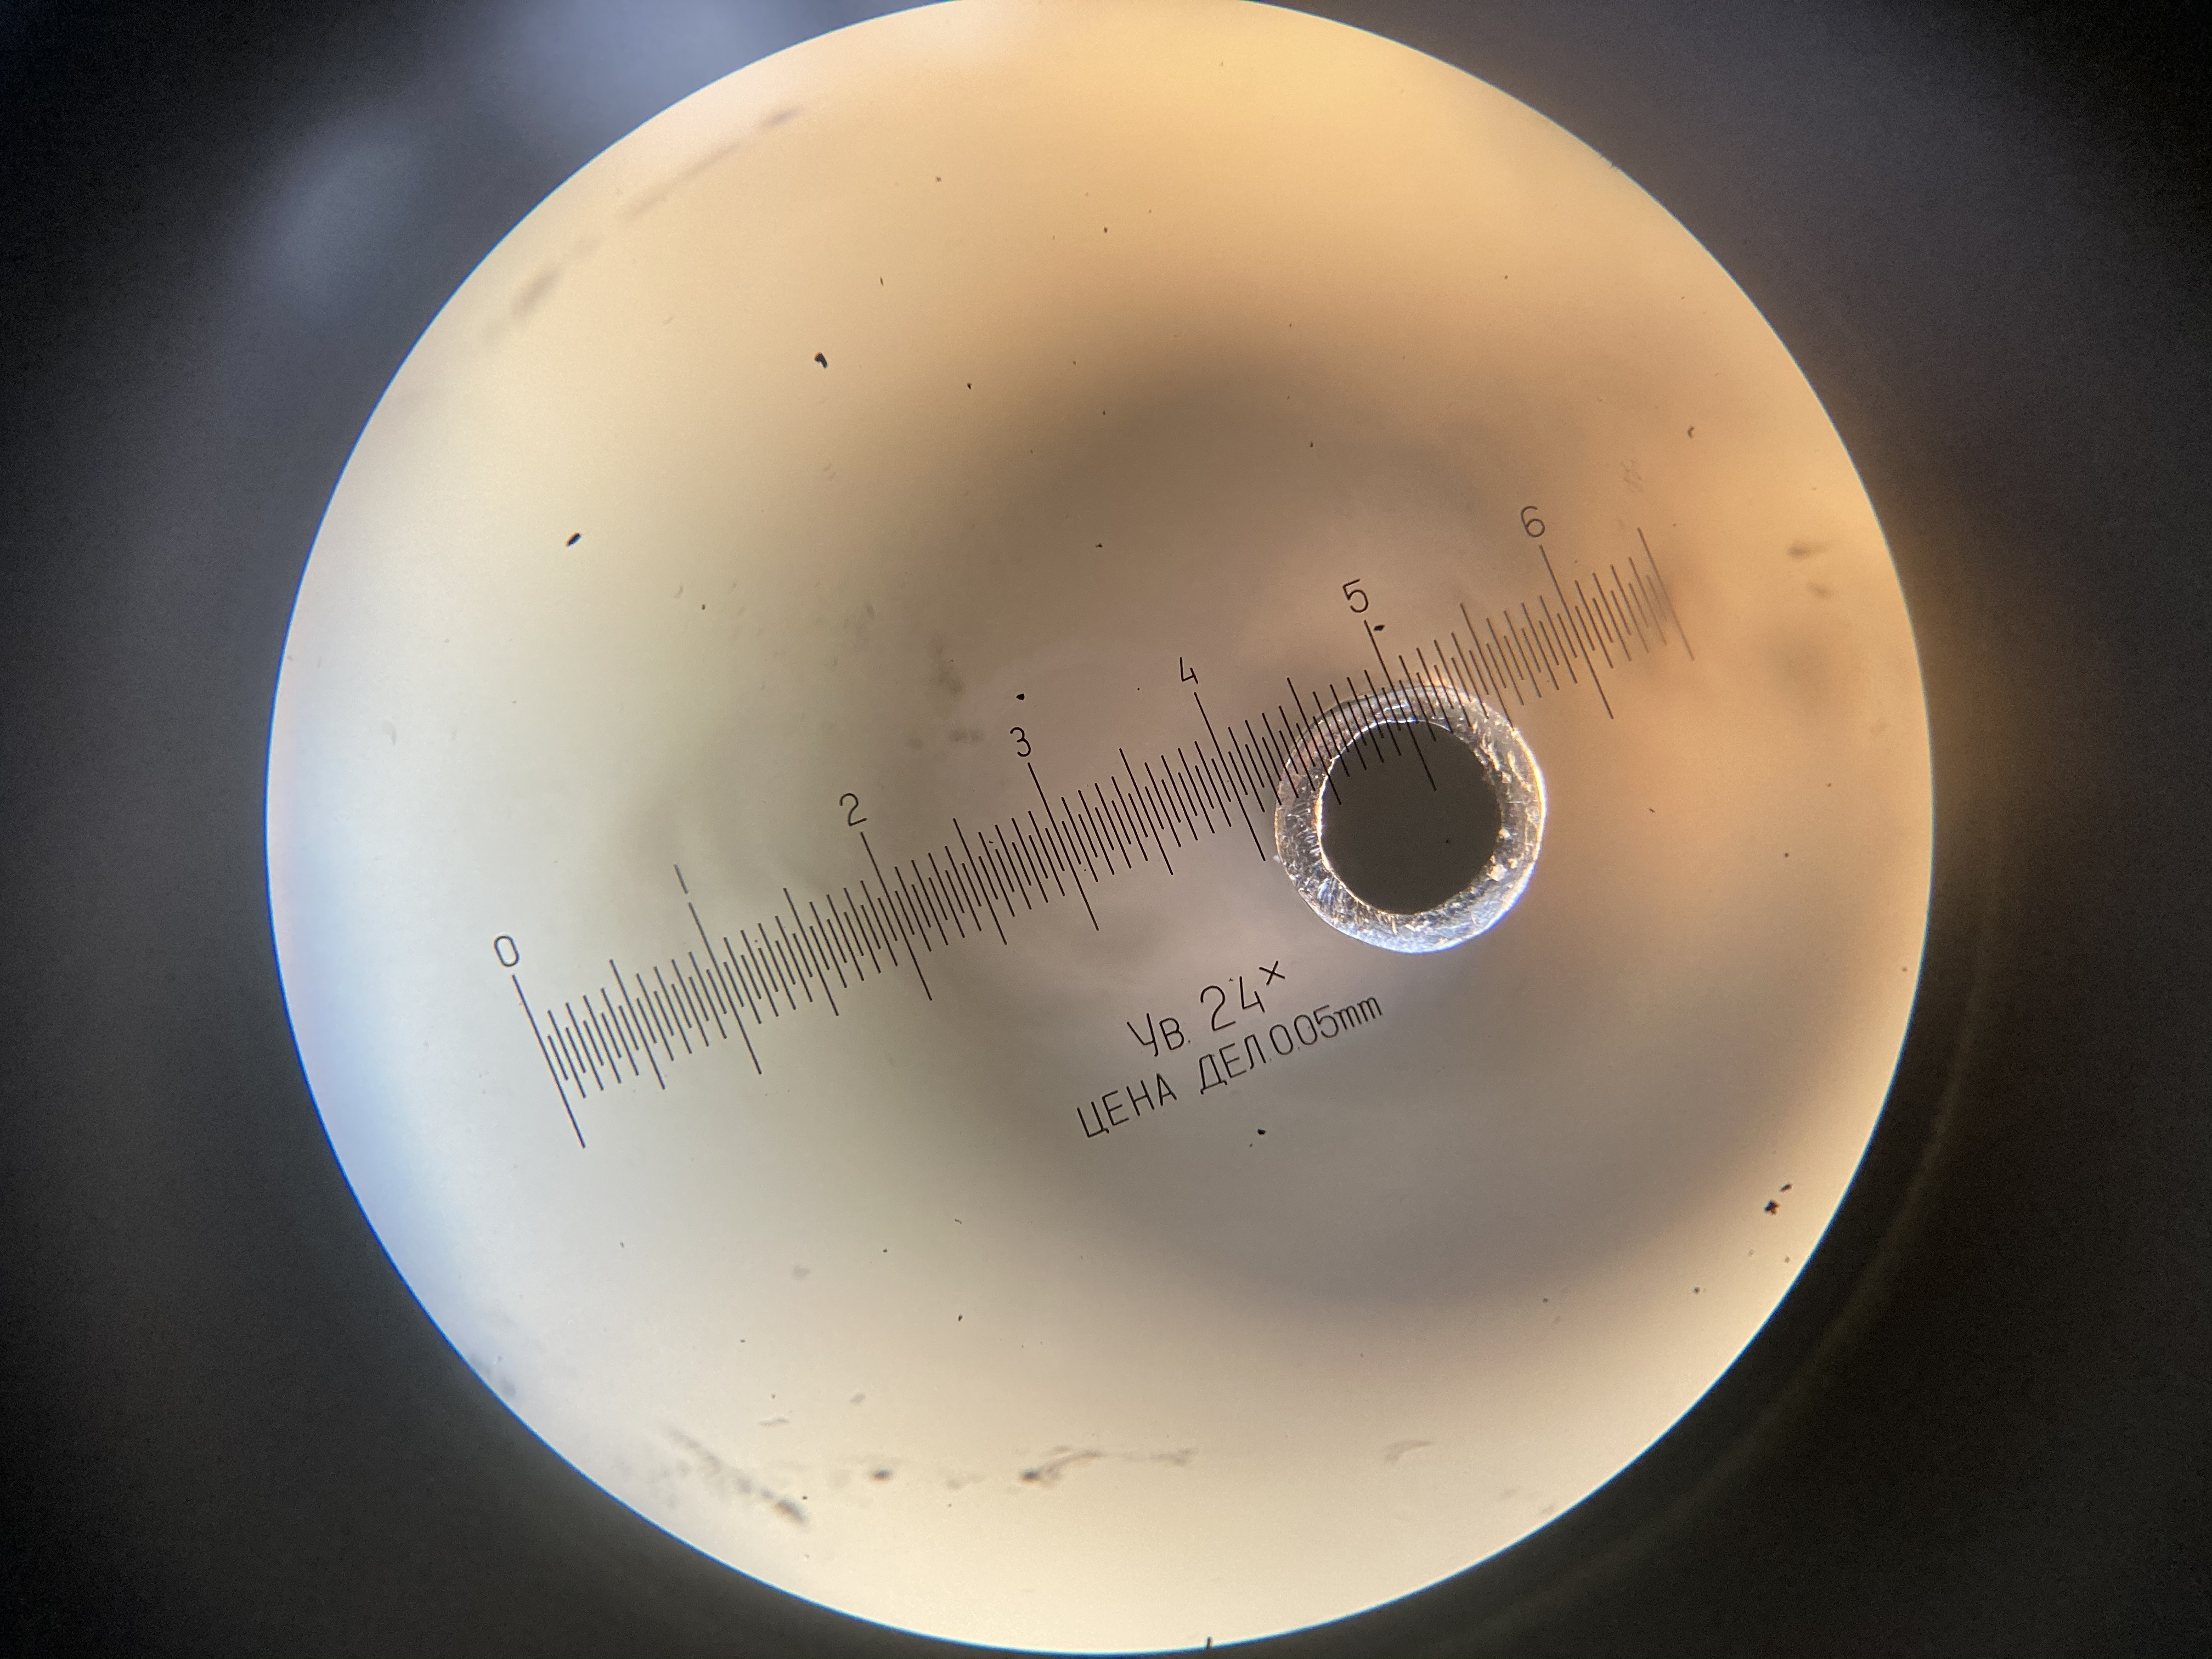
\includegraphics[scale=0.08]{lab251ris2.jpg}}
\caption{\textit{Фотография иглы в микроскопе}}
\end{figure}

\begin{table}[hbt]
\centering
\caption{\textit{Максимальное давление при разных температурах и соответствующмй коэффициент поверхностного натяжения}}
\begin{tabular}{|c|c|c|c|c|c|}
\hline
\textbf{$T, ^{\circ} C$} & \textbf{$\sigma_T, ^{\circ} C$} & \textbf{$P_{max}, Па$} & \textbf{$\sigma_p, Па$} & \textbf{$\sigma(T) \cdot 10^{-7}, Н/м$} & \textbf{$\sigma_{\sigma} \cdot 10^{-7}, Н/м$} \\ \hline
25,2                     & 0,05                            & 269,2                  & 10,05                   & 639                                     & 4                                             \\ \hline
30,2                     & 0,05                            & 264,8                  & 10,05                   & 629                                     & 4                                             \\ \hline
35,2                     & 0,05                            & 261,8                  & 10,05                   & 622                                     & 4                                             \\ \hline
40,1                     & 0,05                            & 260,8                  & 10,05                   & 619                                     & 4                                             \\ \hline
45,1                     & 0,05                            & 253,9                  & 10,05                   & 603                                     & 4                                             \\ \hline
50,1                     & 0,05                            & 250,6                  & 10,05                   & 595                                     & 4                                             \\ \hline
55,1                     & 0,05                            & 247,6                  & 10,05                   & 588                                     & 4                                             \\ \hline
\end{tabular}
\end{table}

\begin{figure}[hbt]\label{risI}
\center{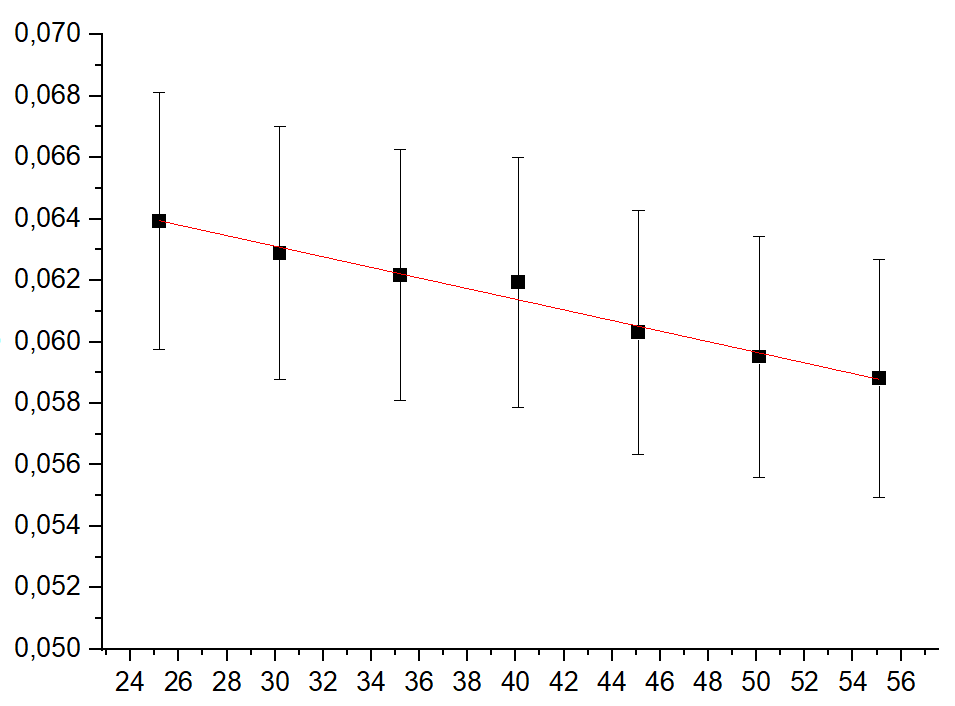
\includegraphics[scale=0.8]{lab251ris3.png}}
\caption{\textit{Зависимость $\sigma(T)$ - коэффициента поверхностного натяжения спирта от температуры. Оси: вертикальная $\sigma$, Н/м; горизонтальная T, $^{\circ}C$}}
\end{figure}

\begin{figure}[hbt]
\center{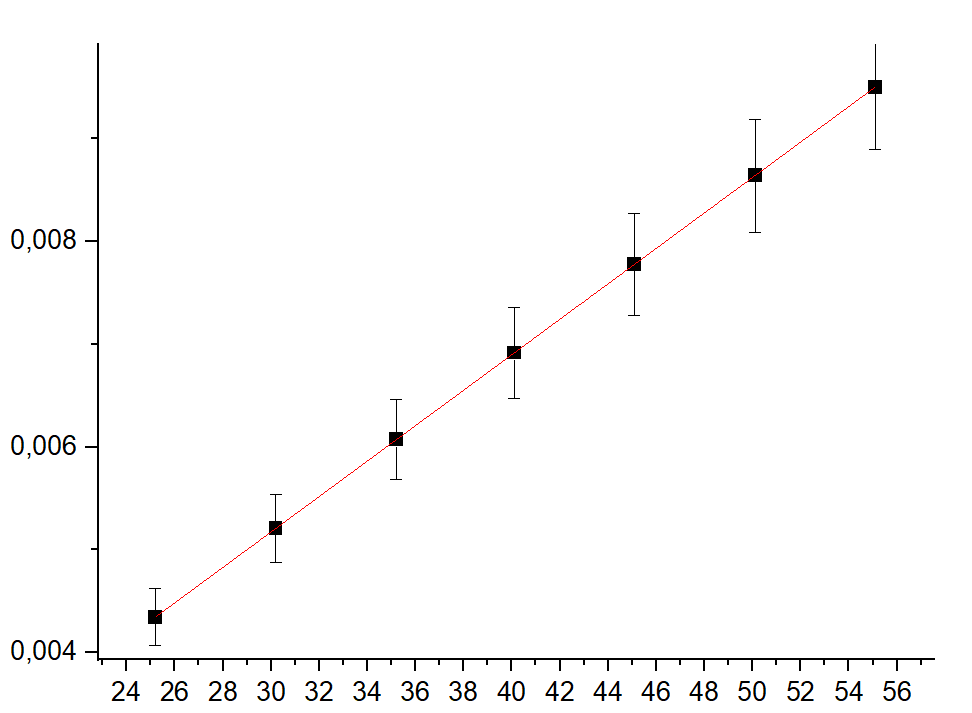
\includegraphics[scale=0.8]{lab251ris4.png}}
\caption{\textit{Зависимость q(T) - теплоты образования единицы поверхности от температуры. Оси: вертикальная $q(T)$, Дж; горизонтальная T, $^{\circ}C$}}
\end{figure}

\begin{figure}[hbt]
\center{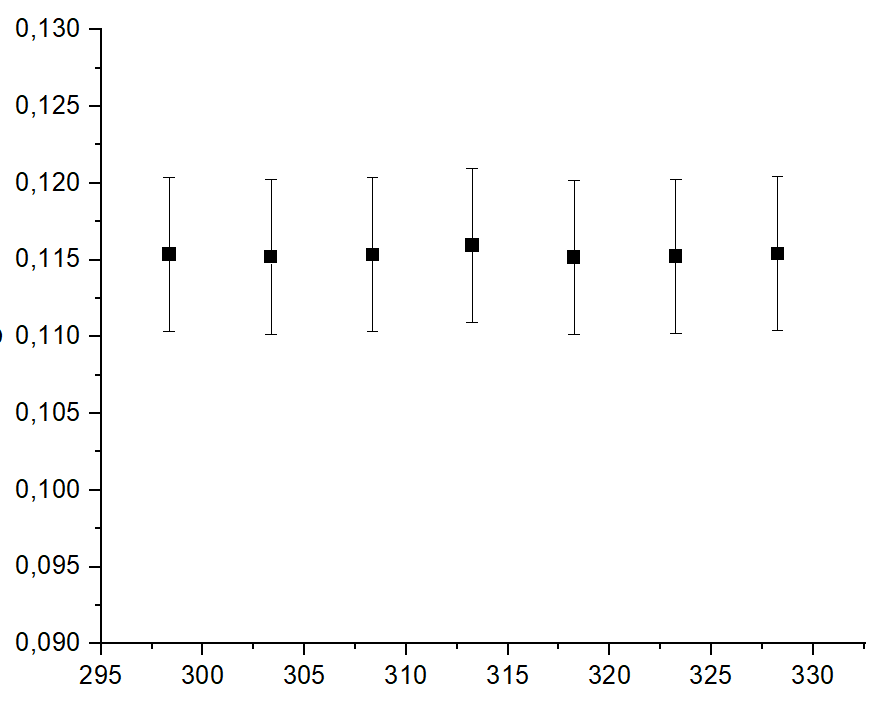
\includegraphics[scale=0.8]{lab251ris5.png}}
\caption{\textit{Зависимость $\frac{U}{F}(T)$ - зависимость поверхностной энергии U единицы площади F от температуры. Оси: вертикальная $q(T)$, Н/м; горизонтальная T, K}}
\end{figure}




\end{document}
